%! TEX root = ../../main.tex

\subsection{Microservices}%
\label{sub:Microservices}

There exist many different definitions of the term \textit{microservice}.
\autocite{DragoniMicroservicesyesterdaytoday2016} defines a microservice to be
a \enquote{cohesive, independent process interacting via messages}. The
definition of \autocite{MikeAmundsenMicroserviceArchitecture2016} also takes
the architectural aspect into account stating that a \textit{microservice
architecture} is a \enquote{style of engineering highly automated, evolvable
software systems made up of capability-aligned microservices}. Regardless of
the specific definition, one common concept becomes clear: A microservice
should be a small independent piece of software that communicates using
messages and that can be deployed autonomously.

This chapter will cover the origins of the microservice architecture, introduce
a practical example of a microservice and outline the problems that need to be
addressed when deploying a microservice.

\subsubsection{History}%
\label{ssub:History}

When designing an application, one option is to use a monolithic architecture.
A monolithic application is developed by one big group of developers and the
source code is maintained inside a single repository. The monolithic
application offers a number of functionalities (also called \textit{services})
that can be consumed. A team of operators is responsible to deploy and manage
the application so that it can be consumed \autocite[p.
584]{VillamizarEvaluatingmonolithicmicroservice2015}. The services of a
monolith can not be executed independently from one another. Hence, a monolith
exists as a single executable artefact \autocite[p.
1]{DragoniMicroservicesyesterdaytoday2016}.

\begin{figure}[H]
\begin{center}
  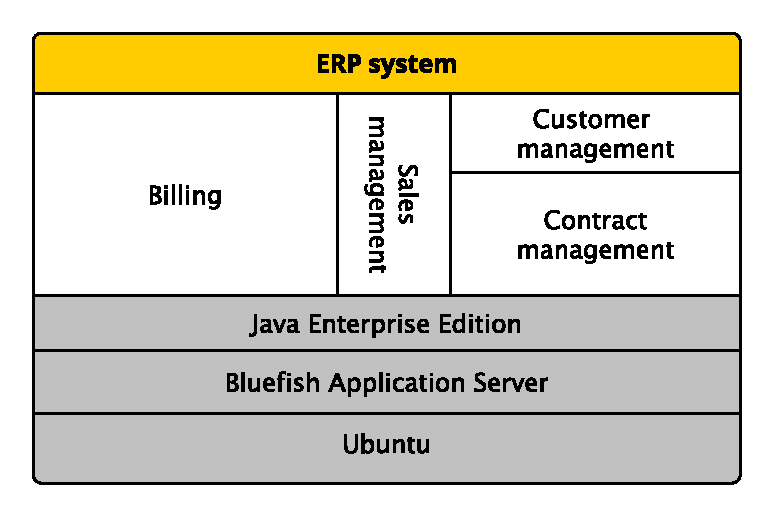
\includegraphics[scale=0.7]{images/figures/monolith_example.pdf}
\end{center}
\caption{An exemplary monolithic \ac{ERP} application based on the Java
Enterprise Edition stack.}%
\label{fig:monolith_example}
\end{figure}

Monolithic applications (as exemplarily portrayed in
figure~\ref{fig:monolith_example}) are hard to deploy in a distributed system
without introducing some kind of middleware that handles the way the monolith
is distributed. Furthermore, monolithic applications suffer additional
drawbacks. Maintaining a monolith can pose a big problem due to its huge code
base and many internal and external dependencies. In addition to this,
deploying a new version can cause major downtimes since the whole application
has to be (re)started. From a development standpoint, monoliths also pose the
problem of restricting the technology stack once it has been defined. This can
produce an environment that is now longer capable being extended with new
services. Lastly, scaling a monolith is not possible indefinitely \autocite[p.
2]{DragoniMicroservicesyesterdaytoday2016}. When scaling an application
\textit{vertically}, resources (e.g.\ \ac{RAM}) are added to the machine
executing the application. Contrary to this approach, when scaling
\textit{horizontally} the application gets distributed onto a number of
machines. This however requires the use of a distributed middleware or code
changes \autocite[Ch. 1.1.1]{LuksaKubernetesAction2017}.

The \ac{SOA} solves a lot of the problems afflicting the monolithic
architecture. Rather than providing all services as part of one application, in
\ac{SOA} the application is split up into multiple small \textit{business
applications} that each offer only a small hand of services. Each business
application is maintained by a specialised development team. The business
applications offer their services to other services or directly to consumers
through a set of protocols; the primarily used protocol is the \ac{SOAP}. The
operation of all business applications is handled by a separate operations team
\autocite[p. 584]{VillamizarEvaluatingmonolithicmicroservice2015}.

Even though the \ac{SOA} approach does solve a lot of problems the monolithic
architecture suffers from, several problems remain. Implementing the \ac{SOA}
into existing and new applications can be difficult resulting in hight costs.
Additionally the technology that is needed to route the requests to the correct
business application is not designed to run inside a modern cloud environment
\autocite[p. 584]{VillamizarEvaluatingmonolithicmicroservice2015}.

The goal of the microservice architecture is to adopt the advantages of the
\ac{SOA} while solving the problems the monolith architecture suffers from
\autocite[p. 584]{VillamizarEvaluatingmonolithicmicroservice2015}.

\autocite{VillamizarEvaluatingmonolithicmicroservice2015} proposes the
questions whether the microservice architecture is a new architectural style or
simply another term for the already existing \ac{SOA}.
\autocite{VillamizarEvaluatingmonolithicmicroservice2015} concludes that the
microservice architecture can be viewed as a subset of the \ac{SOA}. Besides
that it additionally focuses on greater agility. Altogether,
\autocite{DragoniMicroservicesyesterdaytoday2016} defines the microservice
architecture to be a distributed application which \textit{modules} are solely
microservices. The term \enquote{module} is synonymous with the term
\enquote{service} used in the description of the monolithic architecture and
the \ac{SOA}.

Furthermore, the user does not contact any service directly. One or more
gateways receive the user's requests and route them to the correct service.
Depending on the type of user, the requested information are encoded
appropriately by the gateway. An end user might receive a rendered website over
the \ac{HTTP} whereas an \ac{API} call has to be sent via \ac{REST} over
\ac{HTTP}. The operation of said gateway is managed by an independent team
\autocite[p. 585]{VillamizarEvaluatingmonolithicmicroservice2015}. Two common
approaches in this field are \ac{API} gateways and service meshes. Their
properties and respective advantages are further discussed in
\autocite{HariharaSubramanianHandsRESTfulAPI2019}.

In summary it can be said that the microservice architecture constitutes the
natural evolution of software architectural patterns in a distributed system.

\subsubsection{A Concrete Example}%
\label{ssub:A_Practical_Example}

The following example highlights the advantages of microservices in a practical
environment. The example depicts an application that allows users to share
pictures of their pets with other users; hereafter called \textit{PawPic}.
It is a requirement that all users have to be authenticated using an external
\textit{Active Directory} system in order to to view and post pictures.

Following the concept of \textit{cohesion} \autocite[p.
2]{DragoniMicroservicesyesterdaytoday2016}, any service only provides the
functionality that is needed to solve the specific problem it is assigned.
Figure~\ref{fig:microservice_example} proposes a microservice architecture for
the \textit{PawPic} application.

\begin{figure}[H]
\begin{center}
  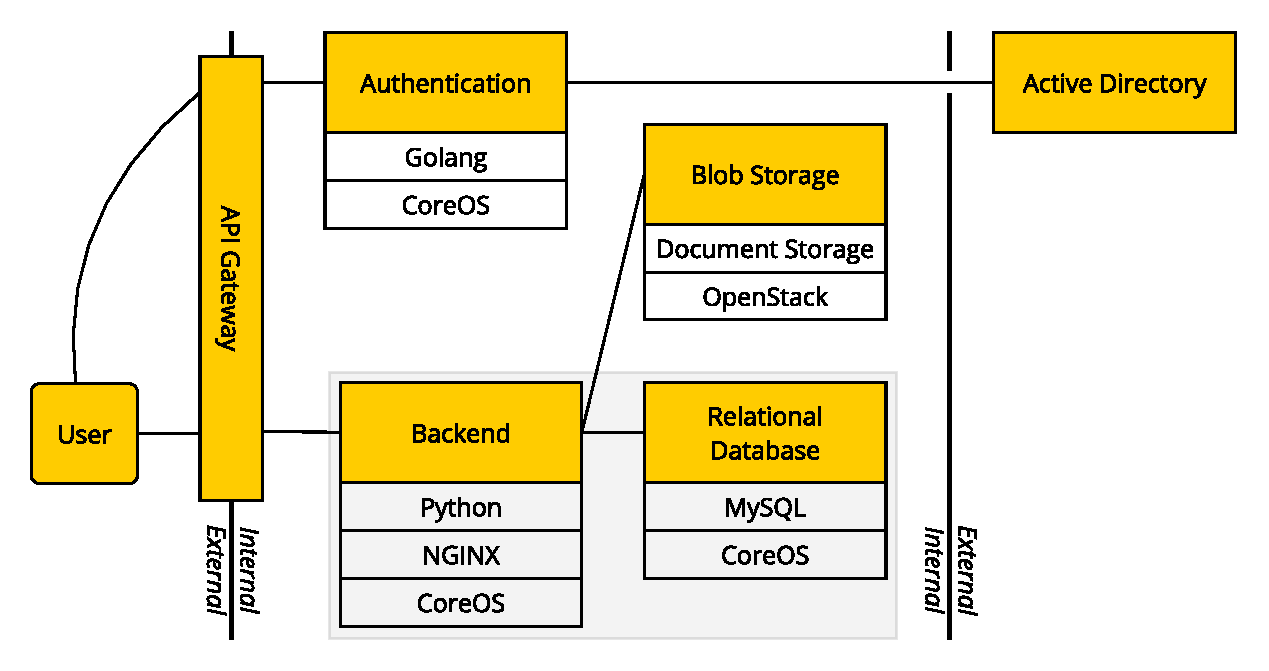
\includegraphics[scale=0.7]{images/figures/microservice_example.pdf}
\end{center}
\caption{A basic microservice architecture example containing three internal
service, one external service and an \acs{API} gateway.}
\label{fig:microservice_example}
\end{figure}

The proposed architecture includes an \ac{API} gateway that handles all requests
targeted at one of the internal services. This only applies to requests by a
user and does not include requests an internal service performs towards an
external service.

The architecture further contains three internal services only two of which can
be directly targeted by the user; the authentication and backend service. The
authentication service's only purpose is to check the user's credentials.
Besides that, the backend service provides the applications main functionality;
to view and share pictures of pets. To fulfil this task, the backend uses a
relational database. The database holds the picture's information and storage
metadata. Both the backend and database are separate services though they are
strongly dependent on one another. Using the storage metadata, the backend is
able to fetch the actual images from the blob storage service and relay them to
the user.

With the introduction of new features it must be decided whether the new
features still solve the problem of viewing and posting pictures of pets. If
this is not the case, a new service must be introduced. This ensures that each
service still follows the concept of cohesion.

The services' technology stacks are fully independent from one another. The
authentication service e.g.\ is written in Golang due to the high performance
the language offers. The backend however is written in Python and runs on top
of a NGINX server. This approach does not lock the developers in one technology
stack that might not suite the problem's needs in the future. In addition,
every service can be scaled independently from one another.

\subsubsection{Deployment -- Choosing the Right Runtime Model}%
\label{ssub:Deployment_Runtime_Model}

Given a fully developed microservice architecture, one question remains: How is
it possible to deploy this bulk of microservices in an efficient way? In a
world filled with monoliths, a specialised operations team would be handed a
piece of software. The operations team then prepares the environment to which
the application should be deployed and tests the release
\autocite{VillamizarEvaluatingmonolithicmicroservice2015}. This process takes a
lot of time and effort and lacks agility; the property microservices strive
for.

The introduction of \acp{VM} helps to speed up the process. Instead of
deploying the application directly to a server's hardware, the application is
deployed within a \ac{VM}. Thanks to this concept, several applications can now
be run on the same hardware. The concept of \acp{VM} does not only benefit
monoliths but also translates to microservices. Instead of running
microservices on multiple physical machines, they can be deployed
independently from one another on the same server.

\acp{VM} introduce more flexibility however they do not constitute the perfect
solution for running a microservice architecture. That is due to the high
resource consumption of \acp{VM}.

\begin{figure}[H]
  \hspace*{\fill}%
  \subfloat[Type2 hypervisor \label{subfig:microserviceType2Hypervisor}]{%
    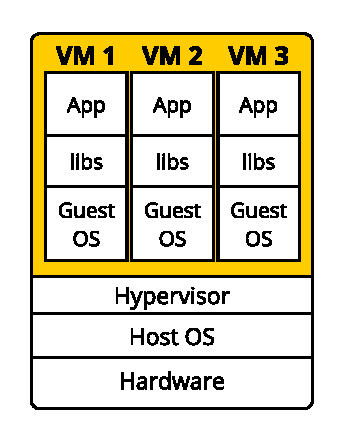
\includegraphics[scale=0.8]{images/figures/hypervisor_type2.pdf}
  }
  \qquad
  \subfloat[(Docker) Container \label{subfig:microserviceContainer}]{%
    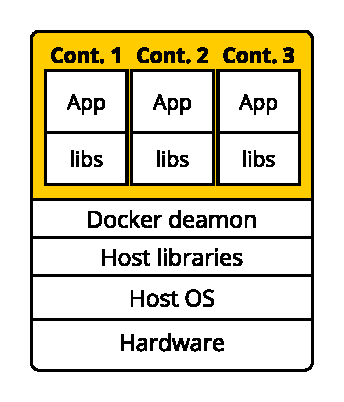
\includegraphics[scale=0.8]{images/figures/container.pdf}
  }
  \hspace*{\fill}%

  \caption[A visual representation of the application runtime models \textit{type2 hypervisor} and \textit{container}.]{A visual representation of the application runtime models \textit{type2 hypervisor} and \textit{container} \autocite[Fig. 1]{CombeDockerNotDocker2016}.}
 \label{fig:hypervisorVsContainer}
\end{figure}

Figure~\ref{subfig:microserviceType2Hypervisor} shows the application runtime
model of a \textit{type2 hypervisor}. In addition to the host \ac{OS}, each
\ac{VM} executes its own full guest \ac{OS}. If this runtime model was chosen
to deploy a microservice architecture, the resource overhead for each
microservice would be major.

The goal is to define a runtime model that encapsulates every microservice as
well as a \ac{VM} executed by a hypervisor does but that is much more light
weight \autocite{SchenkerLearnDockerFundamentals2018}. The container model
depicted in figure~\ref{subfig:microserviceContainer} fits that description.
Rather than needing a full guest \ac{OS} for each application/microservice,
each container only includes the application it is tasked to execute and any
needed libraries. This approach reduces the overhead of each application to a
bare minimum while gaining near bare-metal performance \autocite[Ch.
1A]{CombeDockerNotDocker2016}. In case of the \textit{Docker architecture}
depicted in figure~\ref{subfig:microserviceContainer}, the \textit{Docker
deamon} is responsible for managing all container instances. All of this is
only possible as a result of a few Linux kernel features.
\autocite{CombeDockerNotDocker2016} and \autocite[Ch.
1.2.1]{LuksaKubernetesAction2017} further highlight the security features
needed to make the container runtime model work.

At this point a distinction has to be made: The term Docker refers to a whole
system of functionality. It combines the actual container runtime along with a
reproducible container build process and a central repository, called
\textit{Docker Hub}, where container images can be stored, shared and pulled
from \autocite[Ch. 1B]{CombeDockerNotDocker2016}. Besides that, Docker is not
the only container runtime. Alternatives include \textit{LXC}, \textit{LXD},
\textit{rkt}, \textit{Warden} and \textit{OpenVZ} \autocite[Tab.
1]{CombeDockerNotDocker2016}. Nonetheless all references to containers in this
thesis are references to containers executed by the Docker engine.

\subsubsection{\textit{Dockerizing} a Microservice}%
\label{ssub:Dockerizing_a_Microservice}

Once the actual microservices have been developed, the question arises as to
how they can be deployed with the help of containers. The goal is to execute
one microservice inside at least one container. As already mentioned in chapter
\ref{ssub:Deployment_Runtime_Model}, Docker is equipped with a reproducible
build process for containers. The outcome of such a build process is an
\textit{image}. An image is comprised of the whole file system containing both the
application data as well as all needed libraries and binaries \autocite[Ch.
1]{LuksaKubernetesAction2017}. A container is an instantiation of an image. It
is spawned based on a single image; yet one image can be the base for multiple
containers.

In order to build an image, the developers of a microservice have to define a
\textit{Dockerfile}. The Dockerfile contains all instructions that are needed
by the Docker engine to produce an image. Multiple images built from the same
Dockerfile \textit{should} always be identical because the build process is
deterministic \autocite{DockerBestpracticeswriting}. Their exist a few cases in
which this is not the case. However, they are not relevant to this thesis' work
and thus will not be further examined.

\begin{listing}[H]
\begin{minted}{Dockerfile}
from busybox:1.31.0
RUN echo 'echo "Hello world from BusyBox" \
  $(/bin/busybox | head -1 | cut -d " " -f 2)' > /bin/hello-world
RUN chmod +x /bin/hello-world
ENTRYPOINT exec /bin/hello-world
\end{minted}
\caption{A Dockerfile for building a \textit{hello world} Docker image based on \textit{BusyBox}.}
\label{listing:dockerfile_example}
\end{listing}

Each image has to be built on top of a \textit{base image}. The example image
in listing~\ref{listing:dockerfile_example} is built upon \textit{BusyBox}
which is a very small base image totalling only up to 5 megabyte
\autocite{Communitybusybox2019}.  The instructions inside a Dockerfile are
executed from top to bottom. Each \texttt{RUN} command creates a new
\textit{layer} containing the changes from the executed command. The most
common Dockerfile commands and the issues regarding layering are further
examined in \autocite{DockerBestpracticeswriting}. The command that spans from
line two to three in listing~\ref{listing:dockerfile_example} creates a bash
file that produces this output:

\hspace{1cm} \texttt{Hello from BusyBox 1.31.0}

In line four of the same listing, the \texttt{chmod} utility is used to set the
\textit{execution} permission of the newly created file. This allows the binary
to be executed. The last line of listing~\ref{listing:dockerfile_example} specifies the
\textit{entry point} of the image. The entry point is executed when a new
container is spawned based on this image. The convoluted interrelations between
the \texttt{ENTRYPOINT} and \texttt{CMD} instructions will not be further
examined due to their low relevance to the subject at hand. Their
interrelations are however fully contrasted in
\autocite{DockerDockerfilereferenceEntrypoint}.

\begin{figure}[H]
\begin{center}
  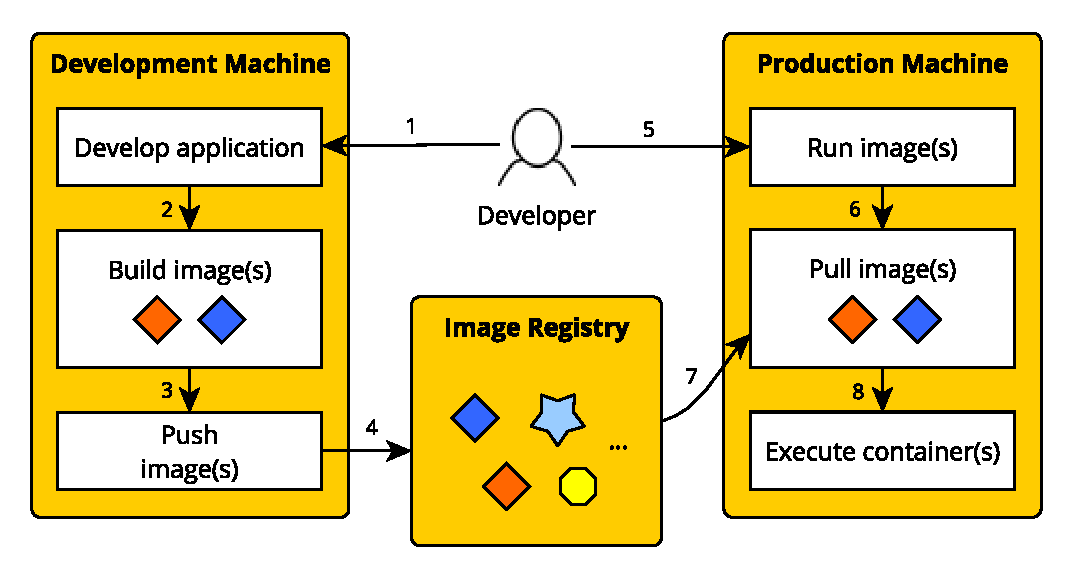
\includegraphics[scale=0.7]{images/figures/docker_workflow.pdf}
\end{center}
\caption[The basic Docker development and deployment workflow.]{The basic Docker development and deployment workflow (adapted from \autocite[Fig. 1.6]{LuksaKubernetesAction2017}).}
\label{fig:docker_workflow}
\end{figure}

All development (step 1 in figure~\ref{fig:docker_workflow}) and image building steps
(step 2 in figure~\ref{fig:docker_workflow}) take place on the developer's machine.
After a development cycle is completed, the developer pushes the newly built
image(s) to a central image repository (step 3 and 4
in figure~\ref{fig:docker_workflow}). Each microservice now exists as a separate image
in the image repository. The production machine then has to be instructed to
run the newly created image(s) (step 5 in figure~\ref{fig:docker_workflow}). This
triggers the Docker daemon (step 6 in figure~\ref{fig:docker_workflow}) to pull the
built images from the image repository (step 7 in figure~\ref{fig:docker_workflow}).
Lastly, all pulled images are executed as a container (step 8
in figure~\ref{fig:docker_workflow}).

The result of this process is a complete microservice architecture running
containerized on a production Docker machine. The process however also reveals
a few problems:
\begin{itemize}
  \item The developer has to tell the production machine that runs the Docker
    engine to execute a new image by hand.
  \item The bigger the microservice architecture gets, the more effort is
    required to run the images on the production machine. This is due to the
    requirement that the developer has to run each image separately. Docker
    provides a mechanism for deploying multiple images at once. The built-in
    method however is not as flexible as the option proposed in the upcoming
    chapter.
  \item In order to distribute images across multiple production machines, some
    \textit{container orchestration} solution is needed. Docker has a built-in
    solution called \textit{Docker Swarm}. Compared to other orchestration
    solutions it is the easiest to understand \autocite[p.
    17]{FabrizioSoppelsaNativeDockerClustering2016}. Next to Docker Swarm, a
    number of alternatives exist. However, all these solutions require a
    separate configuration.
  \item Each image has to be built by the developer on the developers machine.
    The developer is fully responsible for pushing the image to a central image
    repository. This further introduces a security risk because the production
    authentication secrets of the image repository have to be distributed to
    every developer.
\end{itemize}

All in all it can be said that running a containerized microservice
architecture using Docker is a straight-forward process that fails to scale
without further technological improvements.
